\documentclass{article}
% translate with >> pdflatex -shell-escape <file>

% This file is an extract of the PGFPLOTS manual, copyright by Christian Feuersaenger.
% 
% Feel free to use it as long as you cite the pgfplots manual properly.
%
% See
%   http://pgfplots.sourceforge.net/pgfplots.pdf
% for the complete manual.
%
% Any required input files (for <plot table> or <plot file> or the table package) can be downloaded
% at
% http://www.ctan.org/tex-archive/graphics/pgf/contrib/pgfplots/doc/latex/
% and
% http://www.ctan.org/tex-archive/graphics/pgf/contrib/pgfplots/doc/latex/plotdata/

\usepackage{pgfplots}
\pgfplotsset{compat=newest}

\pagestyle{empty}

\begin{document}
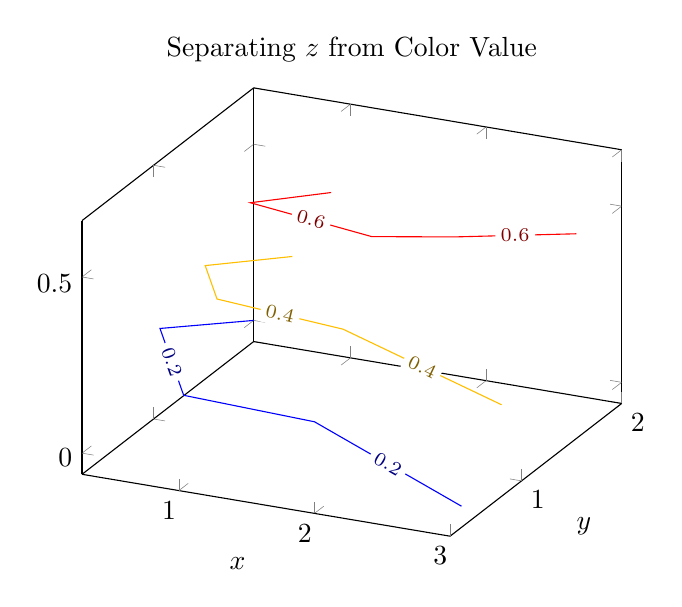
\begin{tikzpicture}
	\begin{axis}[
		title=Separating $z$ from Color Value,
		xlabel=$x$,
		ylabel=$y$,
	]
	\addplot3[contour prepared,
		point meta=\thisrow{level}]
		table {
	 x         y   z   level   
	 0.857143  2  0.4 0.6		
	 1         1  0.6  0.6		
	 2  0.857143 0.6  0.6		
	 2.5  1      0.6  0.6		
	 2.66667  2  0.4  0.6		
	                  		
	 0.571429  2  0.2 0.4		
	 0.666667  1  0.4 0.4		
	 1  0.666667  0.4 0.4		
	 2  0.571429  0.4 0.4		
	 3  0.8       0.2 0.4		
	                  		
	 0.285714  2  0   0.2		
	 0.333333  1  0.2 0.2		
	 1  0.333333  0.2 0.2		
	 2  0.285714  0.2 0.2		
	 3  0.4       0   0.2		
		};
	\end{axis}
\end{tikzpicture}
\end{document}
